\documentclass[conference]{IEEEtran}
\usepackage[colorlinks,allcolors=blue]{hyperref}
\usepackage{amsfonts}
\usepackage{graphicx}
\usepackage{geometry}
\usepackage{dirtree}
\usepackage{enumitem}
\usepackage[table]{xcolor}


\graphicspath{{./images/}}


\begin{document}

    \title{Modeling and Observing Digital Twins with ROS2 and Omniverse}
    \author{\IEEEauthorblockN{Alican Tüzün} 
    \IEEEauthorblockA{University of Applied Sciences Upper Austria\\ Wels, Austria\\ tuzunalican@gmail.com\\}}
    
    \maketitle

    \begin{abstract}
        The paper represents the development of the real system, digital twin prototype (DTP) and digital twin instance (DTI) by strictly following the lifecycle stages of the real system (RS).  
        Furthermore, the development process utilized and leveraged the ROS2 and Omniverse technologies to create a high-fidelity twin of the real system. During the development, several challenges were encountered and addressed, which led to
        valuable observations for the reader. The observations of this study emphasize the significant potential of digital twins as powerful tools for supporting, and potentially even replacing,
        the lifecycle stages of real systems. Consequently, this paper contributes to the scientific and practical knowledge of digital twins. 
    \end{abstract}

    \section{Introduction}\label{section:introduction}
    As new and complex technologies advance to emerge, it becomes progressively difficult to understand and define their core concepts.
    One of the significant current examples in the field of digitalization is the notion of digital twins, which has resulted in numerous definitions~\cite{Review1}, 
    that vary from one derivation to another. Because, even though the terms "digital" and "twin" are easy to grasp, their consolidation develops a new challenging concept, 
    which might be resulted in misunderstanding and misapplication. Therefore, a practical example of a proto, easy-to-model example of the digital twin prototype and instance 
    can significantly improve understanding of the notion of the digital twin.
    
    The digital twin (DT) was proposed in 2002 by Grieves~\cite{Originsofdigitaltwinconcept}, as an ideal form of product life cycle management. The proposal was to create a co-existed information twin of 
    a real system to gather new information to minimize the system needs and waste, such as material, time, and energy. It should be noted that initially this concept was called the mirrored spaced model~\cite{Originsofdigitaltwinconcept}, 
    and later the information mirroring model (IMM)~\cite{GrievesPLMBook,2005ArticleGrievesMichael}. IMM had all the components of today's DTs: a real system (RS), a virtual system, 
    a connection between them, and additionally the virtual simulation~\cite{GrievesPLMBook}.
    However, after co-authoring with Vickers in 2010, the term 'digital twin' was adopted and Grieves simplified the model by excluding the virtual simulation component ~\cite{Originsofdigitaltwinconcept}. 
    
    Since then, there has been a considerable amount of literature published on DTs~\cite{Review1,Review2},
    however, to date, even though Grieves has already given the definition~\cite{Originsofdigitaltwinconcept}, there has been little agreement on the precise definition and application. 
    Numerous authors have considered different definitions, including digital twins as a multi-physics environment~\cite{TheDigitalTwinParadigmforFutureNASAandUSAirForceVehicles}, an equivalent to a product~\cite{SCHROEDER201612}, a digital copy~\cite{SODERBERG2017137}, a cyber component of a Cyber-Physical System~\cite{ADigitalTwinArchitectureReferenceModelfortheCloudBasedCyberPhysicalSystems},
    and many more~\cite{Digitaltwindrivenproductdesignframework,ConferenceonNetworking,Thedigitaltwinimplementationforlinkingthevirtualrepresentationof}. 
    However, if inspected carefully, most of these not only don't coincide with Grieves's definitions but also give some extra aspects to it. 
   
    This absence of agreement exists not only in the literature; it also reaches the industry. This resulted in the development of many different 
    general platforms to construct digital twins~\cite{Ansys,DSDIGITALTWIN}. Furthermore, game engines such as Unity~\cite{Unity} and Unreal Engine~\cite{UnrealEngine} have become popular tools for being an 
    environment for digital twins, and some of them already offer dedicated digital twin platforms~\cite{UnityDT,UnrealEngineDT}. 
    However, while there are some accessible open-source projects~\cite{EclipseDitto,iTwin}, most of the digital twin platforms today are not free to use, 
    which makes it harder to acquire practical knowledge about digital twins. 

    To address the challenges associated with the accessibility and comprehensibility of the notion of digital twins, the author presented the
    process of assembling a real system along with a digital twin prototype (DTP)~\cite{Originsofdigitaltwinconcept}and digital twin instance (DTI)~\cite{Originsofdigitaltwinconcept}, both being forms of DT, 
    by following adopted lifecycle models. Furthermore, the author presented the observations, including the challenges and solutions encountered during the process.

    During the implementation, the author utilized Omniverse~\cite{Omniverse} as a digital twin environment (DTE)~\cite{Originsofdigitaltwinconcept} and used ROS2 (Robot Operating System 2)~\cite{ROS2}
    as a sensor and communication middleware and gave behavior to the real system. An HC-SR04 ultrasonic sensor~\cite{HCSR04}, Raspberry Pi 4 (RPI4)~\cite{RPI4}, 
    basic electronic components (Table~\ref{tab:Hardware}) and several third-party libraries have been used to construct the real system. 

    \section{Method}\label{section:Method}
    To start the process of developing the digital twins and real system (RS), first, a digital prototype (DTP) 
    representing the possible form of the RS, also called a selected prototype, was developed. 
    Second, the physical components of the RS relative to the DTP were assembled. 
    Subsequently, a connection between the RS and the digital twin instance (DTI) was established, 
    resulting in the capturing of information about the product throughout the remaining lifecycle stages.

    Nonetheless, the Digital Twin (DT) is a compendium of product information and evolves through the entire lifecycle of the product. 
    Therefore, it was important to recognize the DTP and DTI's lifecycles, which most of the time run in parallel with the product lifecycle.

    Therefore, the author explored different lifecycle frameworks and standards~\cite{ISO/IEC/IEEE12207,ISO/IEC/IEEE15288,ISO/IEC/IEEE24748-1:2018} and adapted the lifecycle models 
    from ISO/IEC 24748-1 to the notion of digital twins (Figure~\ref{fig:LIFECYCLE}). 
    These frameworks include the stages of  Concept, Development, Support\&Maintenance, and finally Retirement~\cite{ISO/IEC/IEEE24748-1:2018}(Figure~\ref{fig:LIFECYCLE}). 
    However, to effectively demonstrate the construction of the digital twins, the author presented the creation of the DTP and DTI from the perspective of the real system's lifecycle stages. 
    This approach involved an additional stage called production, which includes the process of production of the RS~\cite{ISO/IEC/IEEE24748-1:2018}(Figure~\ref{fig:LIFECYCLE}).

    It should be noted that, in the ideal world, there would be no need for a development or a concept phase 
    for the RS. However, currently, it is not yet feasible to completely digitalize every aspect of the real system, 
    hence DTI and DTP were used to assist the RS through its lifecycle by transforming atoms to bits~\cite{BeingDigital}.

    \begin{figure}[htbp]
        \centering
        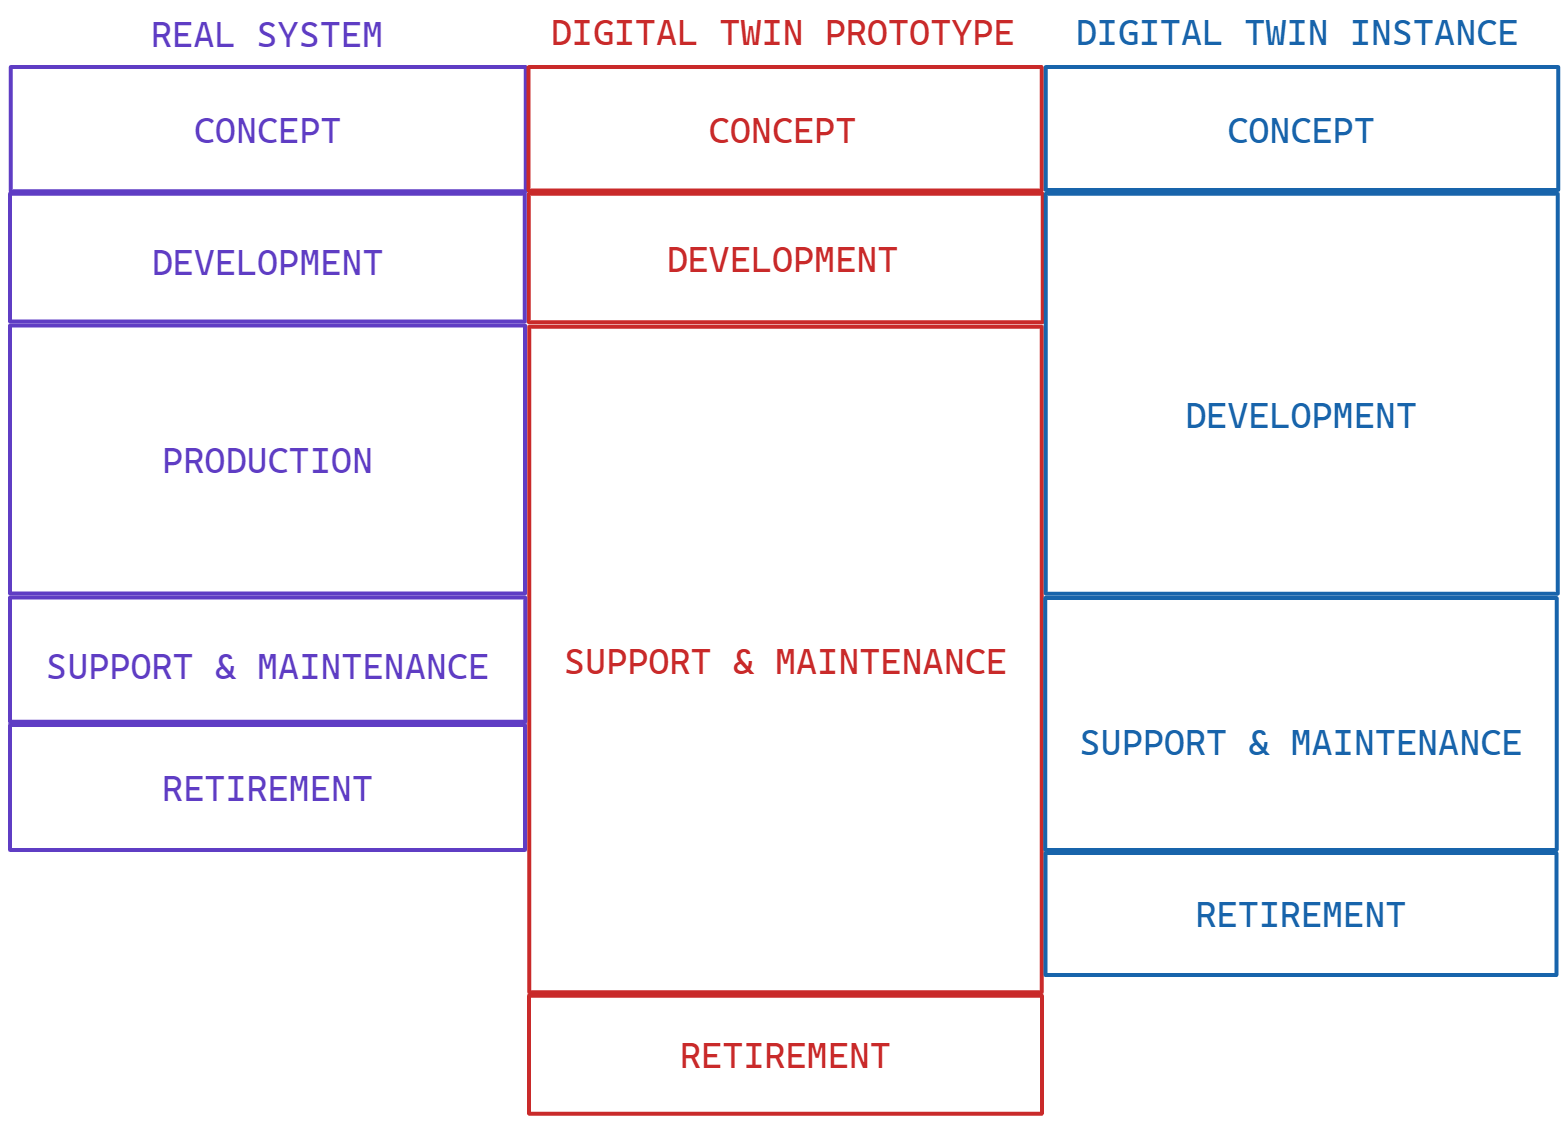
\includegraphics[width=0.45\textwidth]{LIFECYCLE.png}
        \caption{All three lifecycles of RS, DTP, and DTI have been illustrated in order with three different colours.}\label{fig:LIFECYCLE}
    \end{figure}
    
    \subsection{Concept Stage}
    This stage was responsible for exploration, fact-finding, and initial planning while considering the economic, technical, and strategic aspects of the system, in alignment with the desires of the stakeholders. 
    
    To ensure efficiency and productivity, a fast-paced requirement engineering approach was applied, which resulted in the identification of functional and quality requirements, 
    as well as constraints for the DTP, DTI, and RS. Once the requirement analysis was done, and the necessary approvals were obtained, the RS proceeded to the Development Stage. 
    
    \subsection{Development Stage}
    During the development stage, the requirements and design solutions for each system were transformed into feasible products which were used in the following stages of the lifecycle.
    The primary objective of this stage was to develop hardware and software models as well as their corresponding interfaces. 
    These developed models were first analyzed and later verified, and validated. 

    Even though the inclusion of information about the assembly and production planning, maintenance and support procedures as well as retirement considerations,
    and various other aspects should be ideally present in this stage, they were not included in this study due to time and budget constraints. 

    As a result of this stage, the RS was digitally developed and assembled within the DTE as a DTP. This DTP was prepared to assemble the physical components of the RS in the physical,
    observable environment. After the verification and validation process of the developed RS within the DTE was finished, RS proceeded to the Production Stage.

    \subsection{Production Stage}
    The production stage of the RS was constrained by the development stage of the DTP, which progressed with the assistance of  DTP in the observable environment.  
    As an outcome, the RS was initialized in the observable world and was ready for operation during the support and maintenance stage. However, another constraint, the development stage of the DTI, 
    constrained this initiation(Figure~\ref{fig:LIFECYCLE}). Therefore, the development of the DTI was completed before the initiation of the support and maintenance stage of the RS. 
    After the development, the connection between the DTI and RS was established, tested, and evaluated to ensure data capture during the operation.

    \subsection{Service and Maintenance Stage}
    After the production stage, the RS and DTI started to function simultaneously. This functionality or rather a behavior was 
    demonstrated to both technical and non-technical individuals, and this way, the usage of the system was simulated. 
    However, the feedback and assessment from these individuals, such as the quality of the system relative to the user perspective, was out of 
    scope for this paper and hence was not included.  Furthermore, since there was no need for modifications while using/operating the system, 
    as a result, maintenance considerations were excluded. As an outcome of this stage, the real system was ready to be put out of service, in other words, was ready to retire.

    \subsection{Retirement Stage}

    At this stage, the RS was decommissioned and the reusable parts were collected. Simultaneously, DTI and DTP were commencing to service state as the product retired. 
    Since there was no significant waste generated, there was no need for a disposal process.   

   
    \section{Implementation}\label{section:implementation}

    By following the lifecycle framework in Section~\ref{section:Method}, the author ended up using various hardware (Table~\ref{tab:Hardware}) and software tools to conceptualize, 
    develop, produce, operate, and retire the RS along with the DTI and DTP.
    
    \begin{table}[htbp]
        \caption{List of hardware which was used during the development of the RS.}\label{tab:Hardware}
        \begin{tabular}{c c}
        \textbf{Quantity} & \textbf{Item} \\
        \hline
        1 & Raspberry Pi 4 \\
        1 & Raspberry Pi 4 Adapter \\
        1 & RTX Graphics Card 2060 \\
        1 & Prototype Breadboard \\
        1 & Micro SD Card \\
        1 & HC-SR04 Ultrasonic sensor \\
        3 & Light Emitting Diode(LED) \\
        5 & 330 Ohm Resistors \\
        20 & Jumper Cables \\
        \end{tabular}
        \end{table}
    
        
    \subsection{Implementation of the Concept Stage}
    For the concept stage, first, the author focused on the requirement analysis and gathered the requirements for the potential system. Software tools like Obsidian, coupled with the Excalidraw community plugin, 
    were used to conceptualize the systems and most importantly used for the documentation of the requirements.   

    Second, the initial requirements were gathered, listed, and finally categorized into three different groups (Table~\ref{tab:Requirements}).  Later, several prototyping activities were conducted both digital and physical. 
    Later, requirements were elicitated and reworked with the gathered knowledge through prototyping, which resulted in a feasible solution with the selected components to develop a digital twin 
    prototype within the Omniverse. However, it's worth noting that, 
    even though the requirements for the DTE were important, they were not considered due to the simplicity of the project. 

    \begin{table}[htbp]
        \centering
        \caption{List of requirements, bold formatted ones represent the elicited requirements. RP stands for the requirements of the DTP, RI stands for the requirements of the DTI, and RS stands for the requirements of the RS.}
        \label{tab:Requirements}
        \begin{tabular}{p{1cm} p{5.7cm}}
            \textbf{ID} & \textbf{Requirement} \\
            \hline
            RP 1.1 & Digital Twin Prototype should have high fidelity. \\
            RP 1.2 & Digital Twin Prototype must be free to build. \\
            RP 1.3 & Digital Twin Prototype should twin the behavior of the notifications.\\
            \textbf{RP 1.4} & \textbf{Digital Twin Prototype should have Red, Green, and Blue LEDs.}\\
            RI 1.1 & Digital Twin Instance should have high fidelity.\\
            RI 1.2 & Digital Twin Instance must be free to build.\\
            RI 1.3 & Digital Twin Instance should twin the behavior of the notifications with the real system in real-time.\\
            \textbf{RI 1.4} & \textbf{Digital Twin Instance should have Red, Green, and Blue LEDs.}\\
            RS 1.1 &  The real system should cost no more than 200 euros. \\
            RS 1.2 & The real system should notify the user if the digital twin instance is active after 3.5 secs. \\
            \textbf{RS 1.2.1} & \textbf{The real system should have one Blue LED lamp for the RS 1.2.} \\
            RS 1.3 & The real system should notify the user if something is within the 10 cm at the front of the HC-SR04 ultrasonic sensor. \\
            \textbf{RS 1.3.1} & \textbf{The real system should have one Red LED lamp for the RS 1.3.} \\
            RS 1.4 & The real system should notify the user if there is nothing within the 10 cm at the front of the HC-SR04 ultrasonic sensor. \\
            \textbf{RS 1.4.1} & \textbf{The real system should have one Green LED lamp for the RS 1.4.} \\
            RS 1.5 & The real system notifications should be visible in industrial real-time, meaning less than 10 Ms.\\
            RS 1.6 & The real system notifications should be visible at night.\\
            RS 1.7 & The real system should be able to connect to a Wi-Fi network for remote monitoring and control.\\
            RS 1.8 & The real system software should be free to use.\\
            RS 1.9 & The real system should be compatible with the selected digital twin environment.\\
            RS 1.10 & The real system should have a microcontroller to give it controllability.\\
        \end{tabular}
    \end{table}


    \subsection{Implementation of the Development Stage}
    To develop a DTP of the planned RS, two different software programs were used for two different purposes including Fusion 360, a 
    Computer-Aided Design software, and Blender, a 3D-Graphics software. Subsequently, the developed DTP was integrated into the Omniverse, 
    and its behavior was given through the ROS2 node (Figure~\ref{fig:DTP}).

    First, pre-existing digitalized possible RS components were sourced from the internet~\cite{GrabCAD} and were modified for utilization. 
    The components that were not found, such as jumper cables, were developed by the author in the Fusion 360 (Figure ~\ref{fig:DTP}). Once all the required components 
    were available and the model reached the desired fidelity level, 
    detailing was stopped and the individual parts were digitally assembled. Lastly, the assembled digital model was converted to a .fbx file format.
    
    After the conversion, the Blender was used, to convert a .fbx file to a .usd file format with the intention of importing into the DTE. However, before the conversion, 
    several adjustments were made to the .fbx file to fix issues, such as corrupted visuals and inherited hierarchy problems, which occurred due to the insufficient performance of the conversion tools. 

    Furthermore, the headless version of  Ubuntu 20.04 was installed on a micro-SD card, and inserted into the RPI4. Second, the cryptographic network protocol, the secure shell(SSH) 
    was used to connect the RPI4 to a local computer running Ubuntu 20.04. Subsequently, the Robot Operating System 2 (ROS2) version "Foxy" was installed on both the RPI 4 and the local computer. 
    Lastly, to access and control the General Purpose Input/Output (GPIO) pins of the RPI4, the Wiring Pi library was installed on the RPI4.

    ROS2 was used as a sensor and communication middleware to give behavior to the real system components as well as to digital twin instances. Therefore, a custom package was developed with
    C++ programming language to acquire data from the ultrasonic sensor and control the state of three LEDs. This behavior was integrated into a single node, which was executed with a single-thread executor. 
    Lastly, the ROS2 node run and the desired behavior of the real system were observed in the digital twin prototype to ensure that the three LEDs were giving all possible states of the RS.

    To initialize the DTE, Isaac Sim was installed on a local computer using the Omniverse launcher. Once the installation was completed, the correct ROS2 bridge was selected. 
    At this step, it was important not to source the ROS2 Workspace within the same terminal that Isaac Sim was operating, such as through automatic sourcing via bashrc, to prevent potential compilation errors. 

    After the initialization, the modified .usd file was imported into the Omniverse. 
    After the import, a visual inspection of the individual parts was then conducted, to ensure its fidelity. Later,  needed adjustments and modifications were made. 

    Next, to integrate the behavior, a visual scripting tool in Omniverse has been used with the integrated ROS2 bridge. Later behavior of the LEDs was tested visually, 
    and needed corrections and modifications were made. As a consequence, the desired level of fidelity of the DTP, within the DTE was reached (Figure~\ref{fig:DTP}), signifying the success of the process.

    \begin{figure}[htbp]
        \centering
        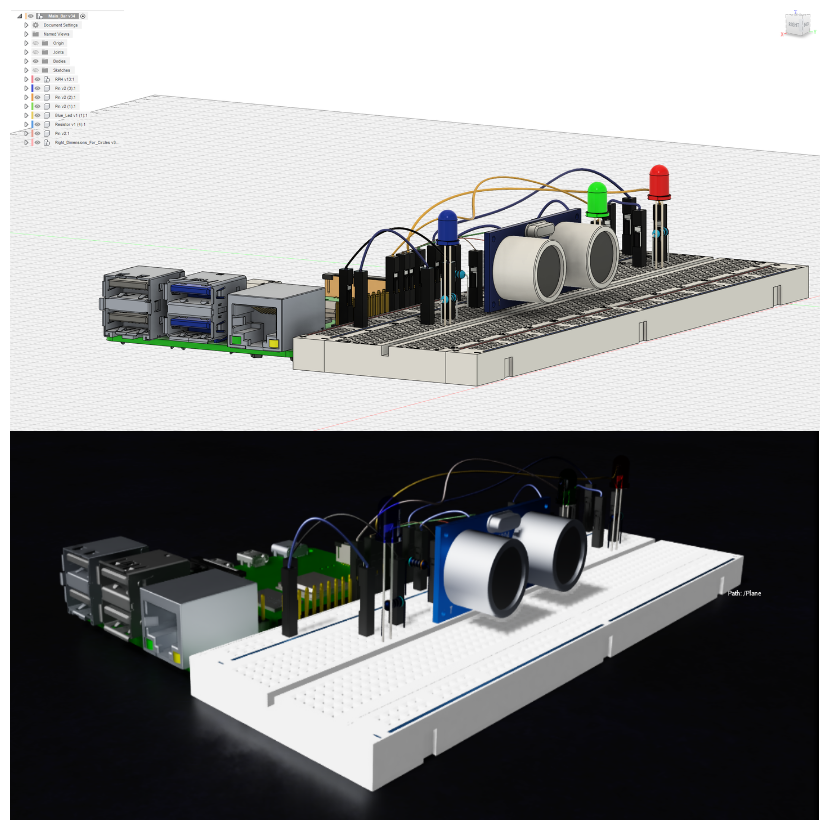
\includegraphics[width=0.45\textwidth]{Left.png}
        \caption{The upper image displays the .step file within the Fusion 360, while the lower image presents the integrated .usd file within Omniverse}\label{fig:DTP}
    \end{figure}
  

    \subsection{Implementation of the Production Stage}

    First, the components were assembled on the prototype breadboard in accordance with the DTP. Next, circuit components were connected with the jumper cables to the appropriate GPIO, ground, and power pins of RPI4 
    (Figure~\ref{fig:DTP}). 

    After the assembly, the DTI interfaces were developed and the ROS2 node from the DTP was copied and later modified, o connect the RS to the DTI. It should be noted that only 
    the behavior of the LEDs was twinned and not the other attributes 
    of the RS such as spatial data of the components, which was tested visually.

    After the development of the DTI was finalized, the RS was ready to proceed to the operation in the support and maintenance stage.

    \begin{figure}[htbp]
        \centering
        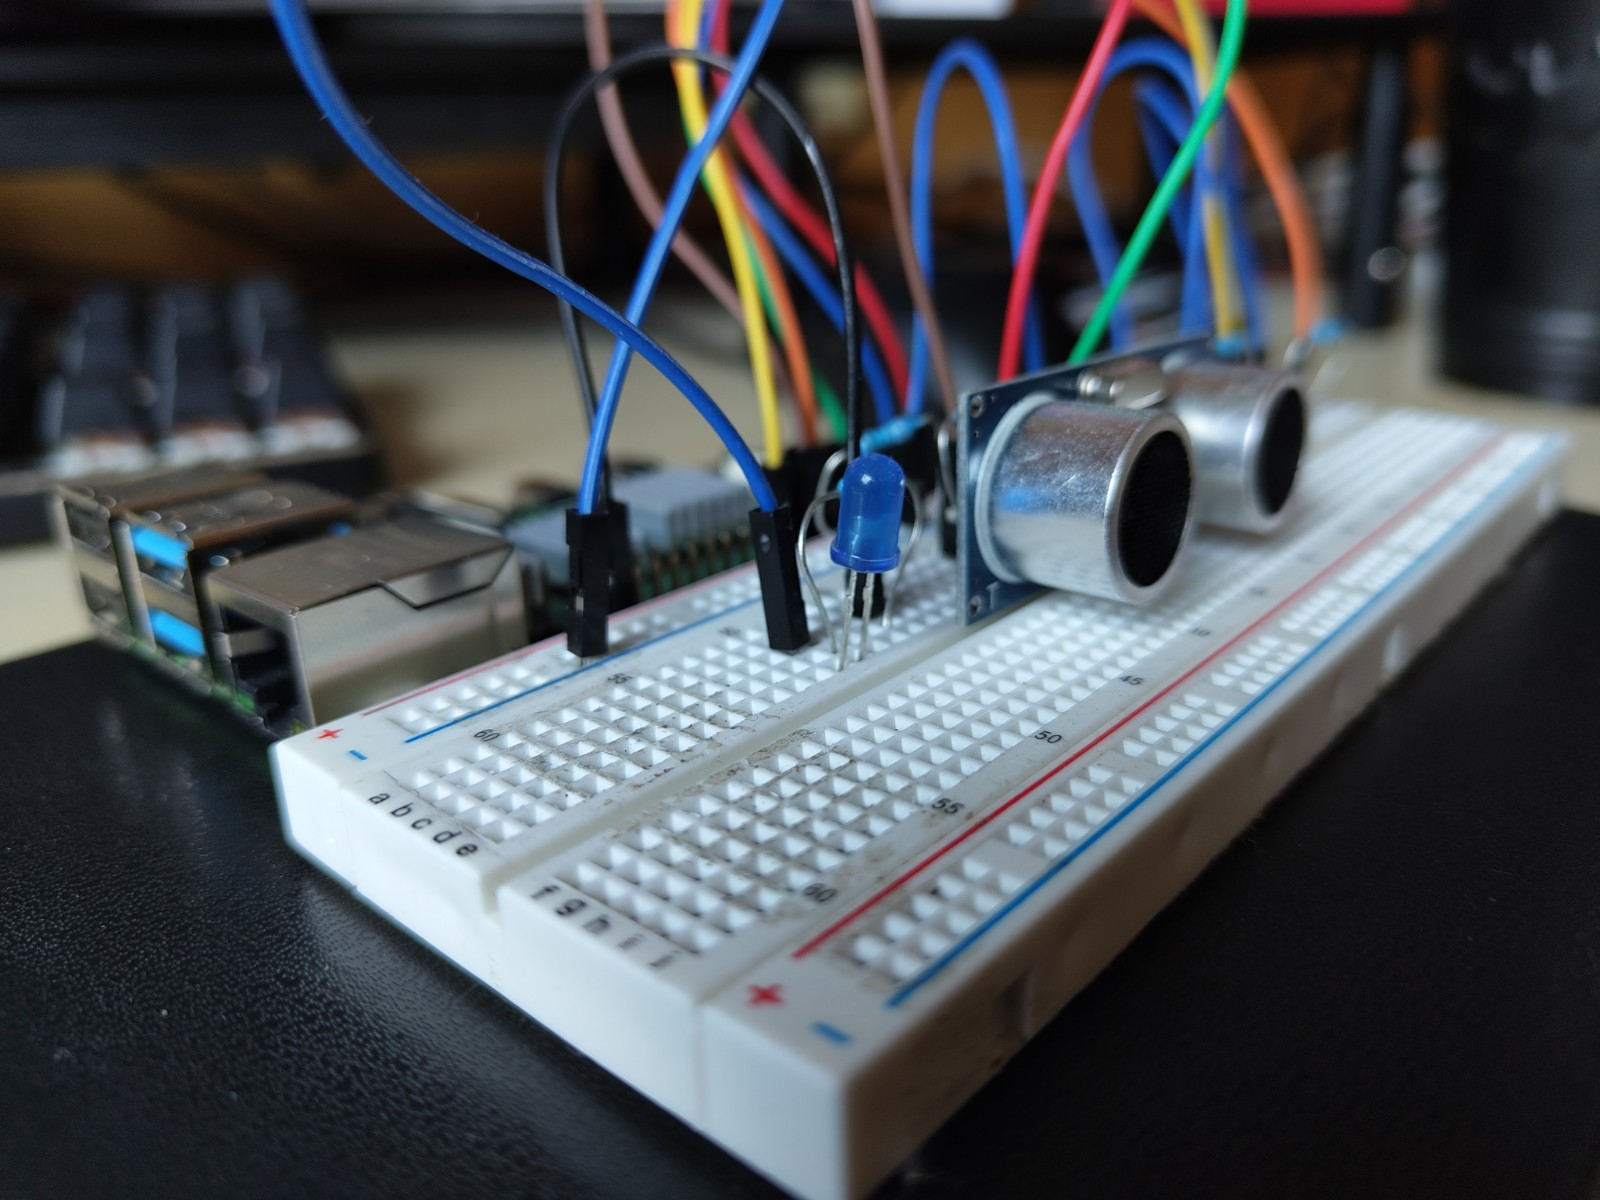
\includegraphics[width=0.45\textwidth]{Assembled.jpg}
        \caption{The image displays the produced or rather assembled real system.}\label{fig:Assembled}
    \end{figure}

    \subsection{Implementation of the Support\&Maintenance and Retirement Stage}
    RS, DTI, and DTP were shown to the stakeholders and their assessment of the quality attributes was written. Later, the RS was decommissioned and disassembled, and DTI and DTP were archived.     

    \section{Observations and Conclusion} 

    To address the challenges associated with the accessibility and comprehensibility of the notion of digital twins, the author followed the lifecycle stages of the real system, 
    while presenting the development of the DTP and DTI. During these stages, there were worthwhile observations, and challenges during the process of creating the digital twins.     

    \subsection{Observations while Creating Digital Twin Prototype}

    The author did not consider the CAD environment as a DTE, instead considered the Omniverse as one. Therefore, in this application, conversion of CAD files to .obj or .fbx and later to .usd file formats were 
    inevitable. However, conversation results showed that a significant amount of model data gets lost, corrupted, or duplicated during the file conversions because of the complexity of 
    the models along with the performance of the converters.

    Therefore to mitigate the data loss, reducing the number of parts by grouping parts together as one solid part and removing the unnecessary details,
    modifying the names of the parts to simple ones, and deleting material properties were helpful and needed. However, some of these processes were irreversible, 
    hence they might reduce the fidelity of the model drastically because of the abstractions through the process.

    Further observations showed that, during the modeling process, non-conventional ways, such as modeling electric cables as 3D in CAD, increased the 
    overall fidelity of the DTP and DTI (Figure~\ref{fig:DTP}).

    Lastly, instead of directly importing the .fbx file directly into the Omniverse, prior to the conversion of the .fbx file to a .usd file, 
    importing the .fbx file into the Blender and making modifications, gave overall better conversion results. This additional process provided more flexibility to manipulate or even correct 
    the corrupted data which occurred during the conversion to .fbx file from .step file in. Fusion 360.

    \subsection{Observations while creating a real system}

    First, the assembly time of the real system was reduced significantly, 
    due to the avaliable spatial and visual data and information from the DTP relative to the traditional methods which lack this kind of information.

    Second, the high-fidelity representation of the components and their connections resulted in a more efficient and flowing assembly process. 

    Furthermore, the utilization of the DTP contributed to the safety of components, during the assembly process and effectively prevented common mistakes. For example, using the exact spatial information of jumper cables from the DTP, prevented the unwanted application of 5V  voltage to GPIO pins through the ultrasonic sensor. This information from the DTP, significantly reduced the possibility of damaging the hardware, in this case, the RPI4. 

    \subsection{Observation while creating and operating the DTI}

    ROS2 played a significant role in the development of flexible DTP and DTI. The nature of  ROS2 allowed for the creation of new nodes with unique functionalities, 
    enabling them to publish and subscribe to messages through the selected topics. For example, the behavior of the Red and Blue LEDs was written in one node and published data to the DTP via 
    the ROS2 bridge to imitate them within the DTE. Later, the same node was used to manipulate the GPIO pins of the RPI4. RPI4 GPIO pins subscribed to the topic, which 
    LED node was publishing on, resulted in putting the GPIO pins in high or low status. This status was later twinned again with the same node in the DTI. 
    This process emerged with simultaneous and real-time publication and subscription of the messages for both the DTP and the DTI by a single node, operating uncoupled.
    
    
    In conclusion, digital twins as a notion, is a powerful tool or rather approach to support and potentially replace the lifecycle stages of the RS, 
    leading to exchange the needed material, energy, and time by using the elucidated information by the digital twins. Furthermore, 
    by utilizing the new and agile technologies, such as machine learning, IoT, VR/AR, robotics, and automation, the information about the product can be exploited even in much more depth. 
    This deeper exploitation of information can open up the possibility for significant enhancements of the DTP's and DTI's in the near future. 

    \bibliography{main}
    \bibliographystyle{plain}
    
\end{document}